\documentclass[a4paper,12pt,twoside]{memoir}

% Castellano
\usepackage[spanish,es-tabla]{babel}
\selectlanguage{spanish}
\usepackage[utf8]{inputenc}
\usepackage[T1]{fontenc}
\usepackage{lmodern} % Scalable font
\usepackage{microtype}
\usepackage{placeins}
\usepackage{float}
\usepackage{lscape}

\RequirePackage{booktabs}
\RequirePackage[table]{xcolor}
\RequirePackage{xtab}
\RequirePackage{multirow}

% Links
\PassOptionsToPackage{hyphens}{url}\usepackage[colorlinks]{hyperref}
\hypersetup{
	allcolors = {red}
}

% Ecuaciones
\usepackage{amsmath}

% Rutas de fichero / paquete
\newcommand{\ruta}[1]{{\sffamily #1}}

% Párrafos
\nonzeroparskip

% Huérfanas y viudas
\widowpenalty100000
\clubpenalty100000

% Imágenes

% Comando para insertar una imagen en un lugar concreto.
% Los parámetros son:
% 1 --> Ruta absoluta/relativa de la figura
% 2 --> Texto a pie de figura
% 3 --> Tamaño en tanto por uno relativo al ancho de página
\usepackage{graphicx}
\newcommand{\imagen}[3]{
	\begin{figure}[!h]
		\centering
		\includegraphics[width=#3\textwidth]{#1}
		\caption{#2}\label{fig:#1}
	\end{figure}
	\FloatBarrier
}

% Comando para insertar una imagen sin posición.
% Los parámetros son:
% 1 --> Ruta absoluta/relativa de la figura
% 2 --> Texto a pie de figura
% 3 --> Tamaño en tanto por uno relativo al ancho de página
\newcommand{\imagenflotante}[3]{
	\begin{figure}
		\centering
		\includegraphics[width=#3\textwidth]{#1}
		\caption{#2}\label{fig:#1}
	\end{figure}
}

\usepackage{graphicx}
\newcommand{\imagenapaisada}[2]{
	\begin{figure}[!h]
		\centering
		\includegraphics[width=1.4\textwidth]{#1}
		\caption{#2}\label{fig:#1}
	\end{figure}
	\FloatBarrier
}

% El comando \figura nos permite insertar figuras comodamente, y utilizando
% siempre el mismo formato. Los parametros son:
% 1 --> Porcentaje del ancho de página que ocupará la figura (de 0 a 1)
% 2 --> Fichero de la imagen
% 3 --> Texto a pie de imagen
% 4 --> Etiqueta (label) para referencias
% 5 --> Opciones que queramos pasarle al \includegraphics
% 6 --> Opciones de posicionamiento a pasarle a \begin{figure}
\newcommand{\figuraConPosicion}[6]{%
  \setlength{\anchoFloat}{#1\textwidth}%
  \addtolength{\anchoFloat}{-4\fboxsep}%
  \setlength{\anchoFigura}{\anchoFloat}%
  \begin{figure}[#6]
    \begin{center}%
      \Ovalbox{%
        \begin{minipage}{\anchoFloat}%
          \begin{center}%
            \includegraphics[width=\anchoFigura,#5]{#2}%
            \caption{#3}%
            \label{#4}%
          \end{center}%
        \end{minipage}
      }%
    \end{center}%
  \end{figure}%
}

%
% Comando para incluir imágenes en formato apaisado (sin marco).
\newcommand{\figuraApaisadaSinMarco}[5]{%
  \begin{figure}%
    \begin{center}%
    \includegraphics[angle=90,height=#1\textheight,#5]{#2}%
    \caption{#3}%
    \label{#4}%
    \end{center}%
  \end{figure}%
}
% Para las tablas
\newcommand{\otoprule}{\midrule [\heavyrulewidth]}
%
% Nuevo comando para tablas pequeñas (menos de una página).
\newcommand{\tablaSmall}[5]{%
 \begin{table}
  \begin{center}
   \rowcolors {2}{gray!35}{}
   \begin{tabular}{#2}
    \toprule
    #4
    \otoprule
    #5
    \bottomrule
   \end{tabular}
   \caption{#1}
   \label{tabla:#3}
  \end{center}
 \end{table}
}

%
% Nuevo comando para tablas pequeñas (menos de una página).
\newcommand{\tablaSmallSinColores}[5]{%
 \begin{table}[H]
  \begin{center}
   \begin{tabular}{#2}
    \toprule
    #4
    \otoprule
    #5
    \bottomrule
   \end{tabular}
   \caption{#1}
   \label{tabla:#3}
  \end{center}
 \end{table}
}

\newcommand{\tablaApaisadaSmall}[5]{%
\begin{landscape}
  \begin{table}
   \begin{center}
    \rowcolors {2}{gray!35}{}
    \begin{tabular}{#2}
     \toprule
     #4
     \otoprule
     #5
     \bottomrule
    \end{tabular}
    \caption{#1}
    \label{tabla:#3}
   \end{center}
  \end{table}
\end{landscape}
}

%
% Nuevo comando para tablas grandes con cabecera y filas alternas coloreadas en gris.
\newcommand{\tabla}[6]{%
  \begin{center}
    \tablefirsthead{
      \toprule
      #5
      \otoprule
    }
    \tablehead{
      \multicolumn{#3}{l}{\small\sl continúa desde la página anterior}\\
      \toprule
      #5
      \otoprule
    }
    \tabletail{
      \hline
      \multicolumn{#3}{r}{\small\sl continúa en la página siguiente}\\
    }
    \tablelasttail{
      \hline
    }
    \bottomcaption{#1}
    \rowcolors {2}{gray!35}{}
    \begin{xtabular}{#2}
      #6
      \bottomrule
    \end{xtabular}
    \label{tabla:#4}
  \end{center}
}

%
% Nuevo comando para tablas grandes con cabecera.
\newcommand{\tablaSinColores}[6]{%
  \begin{center}
    \tablefirsthead{
      \toprule
      #5
      \otoprule
    }
    \tablehead{
      \multicolumn{#3}{l}{\small\sl continúa desde la página anterior}\\
      \toprule
      #5
      \otoprule
    }
    \tabletail{
      \hline
      \multicolumn{#3}{r}{\small\sl continúa en la página siguiente}\\
    }
    \tablelasttail{
      \hline
    }
    \bottomcaption{#1}
    \begin{xtabular}{#2}
      #6
      \bottomrule
    \end{xtabular}
    \label{tabla:#4}
  \end{center}
}

%
% Nuevo comando para tablas grandes sin cabecera.
\newcommand{\tablaSinCabecera}[5]{%
  \begin{center}
    \tablefirsthead{
      \toprule
    }
    \tablehead{
      \multicolumn{#3}{l}{\small\sl continúa desde la página anterior}\\
      \hline
    }
    \tabletail{
      \hline
      \multicolumn{#3}{r}{\small\sl continúa en la página siguiente}\\
    }
    \tablelasttail{
      \hline
    }
    \bottomcaption{#1}
  \begin{xtabular}{#2}
    #5
   \bottomrule
  \end{xtabular}
  \label{tabla:#4}
  \end{center}
}



\definecolor{cgoLight}{HTML}{EEEEEE}
\definecolor{cgoExtralight}{HTML}{FFFFFF}

%
% Nuevo comando para tablas grandes sin cabecera.
\newcommand{\tablaSinCabeceraConBandas}[5]{%
  \begin{center}
    \tablefirsthead{
      \toprule
    }
    \tablehead{
      \multicolumn{#3}{l}{\small\sl continúa desde la página anterior}\\
      \hline
    }
    \tabletail{
      \hline
      \multicolumn{#3}{r}{\small\sl continúa en la página siguiente}\\
    }
    \tablelasttail{
      \hline
    }
    \bottomcaption{#1}
    \rowcolors[]{1}{cgoExtralight}{cgoLight}

  \begin{xtabular}{#2}
    #5
   \bottomrule
  \end{xtabular}
  \label{tabla:#4}
  \end{center}
}



\graphicspath{ {./img/} }

% Capítulos
\chapterstyle{bianchi}
\newcommand{\capitulo}[2]{
	\setcounter{chapter}{#1}
	\setcounter{section}{0}
	\setcounter{figure}{0}
	\setcounter{table}{0}
	\chapter*{\thechapter.\enskip #2}
	\addcontentsline{toc}{chapter}{\thechapter.\enskip #2}
	\markboth{#2}{#2}
}

% Apéndices
\renewcommand{\appendixname}{Apéndice}
\renewcommand*\cftappendixname{\appendixname}

\newcommand{\apendice}[1]{
	%\renewcommand{\thechapter}{A}
	\chapter{#1}
}

\renewcommand*\cftappendixname{\appendixname\ }

% Formato de portada
\makeatletter
\usepackage{xcolor}
\newcommand{\tutor}[1]{\def\@tutor{#1}}
\newcommand{\course}[1]{\def\@course{#1}}
\definecolor{cpardoBox}{HTML}{E6E6FF}
\def\maketitle{
  \null
  \thispagestyle{empty}
  % Cabecera ----------------
\noindent
\includegraphics[width=\textwidth]{cabecera}\vspace{1cm}%
  \vfill
  % Título proyecto y escudo informática ----------------
  \colorbox{cpardoBox}{%
    \begin{minipage}{.8\textwidth}
      \vspace{.5cm}\Large
      \begin{center}
      \textbf{TFG del Grado en Ingeniería Informática}\vspace{.6cm}\\
      \textbf{\LARGE\@title{}}
      \end{center}
      \vspace{.2cm}
    \end{minipage}

  }%
  \hfill\begin{minipage}{.20\textwidth}
    
\includegraphics[width=\textwidth]{escudoInfor}
  \end{minipage}
  \vfill
  % Datos de alumno, curso y tutores ------------------
  \begin{center}%
  {%
    \noindent\LARGE
    Presentado por \@author{}\\ 
    en Universidad de Burgos - \@date{}\\
    \begin{tabbing}
    Tutores: \= Dr. César Ignacio García Osorio\kill
    Tutores: \> Dr. César Ignacio García Osorio\\
    \> Dra. Ana Serrano Mamolar\\
    \end{tabbing}
  }%
  \end{center}%
  \null
  \cleardoublepage
  }
\makeatother

\newcommand{\nombre}{Miguel Ubierna Gutiérrez} %%% cambio de comando

% Datos de portada
\title{DeltaOffers}
\author{\nombre}
\tutor{Dr. César Ignacio Garcia Osorio\\y Dra. Ana Serrano Mamolar}
\date{\today}

\begin{document}

\maketitle


\newpage\null\thispagestyle{empty}\newpage


%%%%%%%%%%%%%%%%%%%%%%%%%%%%%%%%%%%%%%%%%%%%%%%%%%%%%%%%%%%%%%%%%%%%%%%%%%%%%%%%%%%%%%%%
\thispagestyle{empty}


\noindent
\includegraphics[width=\textwidth]{cabecera}\vspace{1cm}

\noindent D. César Ignacio García Osorio y Ana Serrano Mamolar, profesores del departamento de Ingeniería Informática, área de Lenguajes y Sistemas Informáticos.

\noindent Exponen:

\noindent Que el alumno D. \nombre, con DNI 71309923X, ha realizado el Trabajo final de Grado en Ingeniería Informática titulado «DeltaOffers». 

\noindent Y que dicho trabajo ha sido realizado por el alumno bajo la dirección del que suscribe, en virtud de lo cual se autoriza su presentación y defensa.

\begin{center} %\large
En Burgos, {\large \today}
\end{center}

\vfill\vfill\vfill

% Author and supervisor
\begin{minipage}{0.45\textwidth}
\begin{flushleft} %\large
Vº. Bº. del Tutor:\\[2cm]
Dr. César Ignacio García Osorio
\end{flushleft}
\end{minipage}
\hfill
\begin{minipage}{0.45\textwidth}
\begin{flushleft} %\large
Vº. Bº. del co-tutor:\\[2cm]
Dra. Ana Serrano Mamolar
\end{flushleft}
\end{minipage}
\hfill

\vfill

% para casos con solo un tutor comentar lo anterior
% y descomentar lo siguiente
%Vº. Bº. del Tutor:\\[2cm]
%D. nombre tutor


\newpage\null\thispagestyle{empty}\newpage




\frontmatter

% Abstract en castellano
\renewcommand*\abstractname{Resumen}
\begin{abstract}
Actualmente, las convocatorias para el Personal Docente e Investigador y el Personal de Administración y Servicios de las universidades públicas de Castilla y León, se muestran en las páginas web de las respectivas universidades. Cada universidad muestra sus propias convocatorias en su web, esto hace que las correspondientes convocatorias solo estén al alcance de aquellas personas que entran en la web de una universidad especifica.

El trabajo realizado llamado DeltaOffers está compuesto por dos aplicaciones independientes. La primera, se encarga de recopilar mediante \textit{web scraping} todas esas convocatorias de las universidades públicas de Castilla y León y las almacena en una base de datos. Sin embargo, la segunda es una aplicación web que muestra las convocatorias de forma centralizada. Esto amplía enormemente el rango de candidatos en las convocatorias correspondientes. 

Gracias a este proyecto, se puede evitar la ausencia de candidatos para determinadas plazas del PDI y PAS. Además, como la demanda de determinadas convocatorias será mayor, se podrá conseguir personal más cualificado para determinados puestos de trabajo. 

Se puede acceder a la correspondiente página web a partir del siguiente enlace: \href{https://deltaoffers.azurewebsites.net/}{https://deltaoffers.azurewebsites.net/}
\end{abstract}

\renewcommand*\abstractname{Descriptores}
\begin{abstract}
Convocatorias, Personal Docente e Investigador, Personal Administración y Servicios, Universidades, Web Scraping, Cron , Base de datos , Servidores Azure, Página Web, Correo Electrónico, ICalendar.
\end{abstract}

\clearpage

% Abstract en inglés
\renewcommand*\abstractname{Abstract}
\begin{abstract}
Currently, the calls for Teaching and Research Staff and Administration and Services Staff of the public universities of Castilla y León are displayed on the universities' websites. Each university shows its own calls on its website, this means that the corresponding calls are only available to those people who enter the website of a specific university.

The project carried out called DeltaOffers is made up of two independent applications. The first is responsible for collecting all these calls from the public universities of Castilla y León through web scraping and storing them in a database. However, the second is a web application that displays the calls centrally. This greatly expands the range of candidates in the corresponding calls.

Thanks to this project, the absence of candidates for certain PDI and PAS positions can be avoided. Furthermore, as the demand for certain calls will be greater, more qualified personnel will be able to be obtained for certain jobs. 

The corresponding web page can be accessed from the following link: \href{https://deltaoffers.azurewebsites.net/}{https://deltaoffers.azurewebsites.net/}
\end{abstract}

\renewcommand*\abstractname{Keywords}
\begin{abstract}
Calls, Teaching and Research Staff, Administration and Services Staff Universities, Web Scraping, Cron, Database, Azure Servers, Website, Email, ICalendar.
\end{abstract}

\clearpage

% Indices
\tableofcontents

\clearpage

\listoffigures

\clearpage

\mainmatter
\capitulo{1}{Introducción}

Descripción del contenido del trabajo y del estructura de la memoria y del resto de materiales entregados.

\capitulo{2}{Objetivos del proyecto}

Este apartado explica de forma precisa y concisa cuales son los objetivos que se persiguen con la realización del proyecto. Se puede distinguir entre los objetivos marcados por los requisitos del software a construir y los objetivos de carácter técnico que plantea a la hora de llevar a la práctica el proyecto.

\capitulo{3}{Conceptos teóricos}

En aquellos proyectos que necesiten para su comprensión y desarrollo de unos conceptos teóricos de una determinada materia o de un determinado dominio de conocimiento, debe existir un apartado que sintetice dichos conceptos.

Algunos conceptos teóricos de \LaTeX{} \footnote{Créditos a los proyectos de Álvaro López Cantero: Configurador de Presupuestos y Roberto Izquierdo Amo: PLQuiz}.

\section{Secciones}

Las secciones se incluyen con el comando section.

\subsection{Subsecciones}

Además de secciones tenemos subsecciones.

\subsubsection{Subsubsecciones}

Y subsecciones. 


\section{Referencias}

Las referencias se incluyen en el texto usando cite~\cite{wiki:latex}. Para citar webs, artículos o libros~\cite{koza92}, si se desean citar más de uno en el mismo lugar~\cite{bortolot2005, koza92}.


\section{Imágenes}

Se pueden incluir imágenes con los comandos standard de \LaTeX, pero esta plantilla dispone de comandos propios como por ejemplo el siguiente:

\imagen{escudoInfor}{Autómata para una expresión vacía}{.5}



\section{Listas de items}

Existen tres posibilidades:

\begin{itemize}
	\item primer item.
	\item segundo item.
\end{itemize}

\begin{enumerate}
	\item primer item.
	\item segundo item.
\end{enumerate}

\begin{description}
	\item[Primer item] más información sobre el primer item.
	\item[Segundo item] más información sobre el segundo item.
\end{description}
	
\begin{itemize}
\item 
\end{itemize}

\section{Tablas}

Igualmente se pueden usar los comandos específicos de \LaTeX o bien usar alguno de los comandos de la plantilla.

\tablaSmall{Herramientas y tecnologías utilizadas en cada parte del proyecto}{l c c c c}{herramientasportipodeuso}
{ \multicolumn{1}{l}{Herramientas} & App AngularJS & API REST & BD & Memoria \\}{ 
HTML5 & X & & &\\
CSS3 & X & & &\\
BOOTSTRAP & X & & &\\
JavaScript & X & & &\\
AngularJS & X & & &\\
Bower & X & & &\\
PHP & & X & &\\
Karma + Jasmine & X & & &\\
Slim framework & & X & &\\
Idiorm & & X & &\\
Composer & & X & &\\
JSON & X & X & &\\
PhpStorm & X & X & &\\
MySQL & & & X &\\
PhpMyAdmin & & & X &\\
Git + BitBucket & X & X & X & X\\
Mik\TeX{} & & & & X\\
\TeX{}Maker & & & & X\\
Astah & & & & X\\
Balsamiq Mockups & X & & &\\
VersionOne & X & X & X & X\\
} 

\capitulo{4}{Técnicas y herramientas}

Esta parte de la memoria tiene como objetivo presentar las técnicas metodológicas y las herramientas de desarrollo que se han utilizado para llevar a cabo el proyecto. Si se han estudiado diferentes alternativas de metodologías, herramientas, bibliotecas se puede hacer un resumen de los aspectos más destacados de cada alternativa, incluyendo comparativas entre las distintas opciones y una justificación de las elecciones realizadas. 
No se pretende que este apartado se convierta en un capítulo de un libro dedicado a cada una de las alternativas, sino comentar los aspectos más destacados de cada opción, con un repaso somero a los fundamentos esenciales y referencias bibliográficas para que el lector pueda ampliar su conocimiento sobre el tema.



\capitulo{5}{Aspectos relevantes del desarrollo del proyecto}

En este apartado, se van a detallar los aspectos más interesantes del desarrollo del proyecto y los desafíos a los que me he tenido que enfrentar a lo largo del mismo. 

Además, es importante detallar las decisiones que se tomaron en esos momentos de dificultad e indicar de qué manera se solventaron los problemas.

Por otro lado, también voy a indicar en este apartado cual es la arquitectura general del sistema diseñado dado que me parece que es un aspecto interesante dentro del proyecto.

\section{Análisis de las webs de extracción de datos}
En las primeras fases del proyecto, se realizó un análisis de las webs de las Universidades públicas de Castilla y León para estudiar cuales podrían ser los atributos de interés para mostrar en la web del proyecto. Durante este proceso, surgieron varios problemas para la obtención de información. Esto se debió a que cada universidad subía las convocatorias a su web con un formato particular y con unos datos e informaciones particulares. Esto es un problema a la hora de querer montar una web de convocatorias centralizada dado que uno de los aspectos más importantes de una web es la uniformidad de la misma. A continuación, se van a comentar algunos de los desafíos que fueron encontrados durante esta fase.

\subsection{Universidad de Salamanca}
Debido a mi poco conocimiento en cuanto a las convocatorias PDI y PAS, en primer lugar se realizó \textit{web scraping} de un portal de la USAL en el que se publicaban todas las convocatorias pero en el que no se tenía conocimiento si una convocatoria estaba en plazo o no. Esto se debe a que las fechas que comprendían el plazo no estaban publicadas en páginas web sino en documentos PDF. 

Se planteó la posibilidad de realizar PDF scraping de las convocatorias de esta universidad pero tras tiempo de investigación, se descubrió que estos ficheros no seguían un formato unificado.  Finalmente, debido a la imposibilidad de recopilación de datos de la web de la USAL ~\cite{usal:latex} debido a la falta de datos necesarios para la web a desarrollar, se decidió excluir esta universidad del proyecto.

\subsection{Universidad de León}
El realizar el raspado de datos de esta universidad, también fue un reto en el proyecto. Esta universidad mostraba algunas convocatorias en plazo mientras que en verdad ya no estaban abiertas a candidatos (Por ejemplo, ya se habían publicado los listados de admitidos) ~\cite{ule:latex}. Para determinar si una oferta estaba en plazo o no, la única manera era mediante la examinación de los títulos de los PDF adjuntos a una determinada convocatoria. Para ello, se realizó una estructura de datos con las palabras no deseadas con aquellas palabras que, en el caso de localizar alguna en un título ya sabíamos que esa convocatoria no estaba en plazo. 

Esto llevo largos tiempos de análisis para finalmente tan solo acabar detectando las convocatorias que estaban en plazo verdaderamente. Es posible, que en casos futuros, vuelvan a surgir convocatorias fuera de plazo que están detectadas como que si lo son. Para ello, es necesario que si se continúa con el desarrollo de la aplicación, se tenga muy en cuenta este aspecto.

A continuación se va a mostrar un ejemplo en el que se da este caso. En la siguiente imagen, se va a exponer una convocatoria que actualmente está en plazo:

\begin{figure}[H]
    \centering
    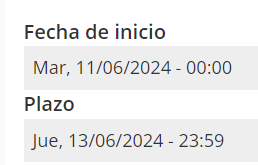
\includegraphics[width=0.4\linewidth]{DocumentacionTFG//img/ConvocatoriaEnPlazoULE.PNG}
    \caption{Convocatoria en plazo ULE}
    \label{fig:enter-label}
\end{figure}

Sin embargo, si nos fijamos en el archivo adjunto a esa convocatoria, aparecerá una resolución de aprobados, lo cual quiere decir que la convocatoria no está en plazo.

\begin{figure}[H]
    \centering
    
\includegraphics[width=0.75\linewidth]{DocumentacionTFG//img/FicheroAdjuntoULE.PNG}
    \caption{Fichero Adjunto a Convocatoria}
    \label{fig:enter-label}
\end{figure}

Con la implementación de la estructura de datos de las palabras no deseadas, esta convocatoria no sería elegida.

\subsection{Universidad de Valladolid}
Al realizar \textit{web scraping} de las páginas web en las que se muestran las convocatorias PDI Y PAS de la Universidad de Valladolid ~\cite{uva:latex}, también surgieron una serie de imprevistos. Esto se debe a que había convocatorias que aparecen en esta web cuyo estado indicaba que estaba 'EN PLAZO' pero si nos fijamos en las fechas de las mismas en verdad no lo están.

\begin{figure}[H]
    \centering
    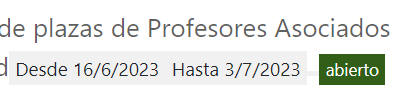
\includegraphics[width=0.75\linewidth]{DocumentacionTFG//img/EjemploConvocatoriaIncorrectaUVA.PNG}
    \caption{Estado Convocatoria Incorrecto}
\end{figure}

Esto fue algo que no percibí en la primera etapa del proyecto, posteriormente, decidí arreglarlo para que las ofertas se mostrasen en plazo con exactitud mediante la comparación de las fechas del plazo con la fecha actual.

Otro de los problemas, fue que, en numerosas convocatorias de la Universidad de Valladolid, había campos vacíos, esto hizo que en algunas convocatorias que por ejemplo no indicaban cuales eran su fecha de inicio de plazo y su fecha de fin, se tuviesen que determinar por cerradas.

\begin{figure}[H]
    \centering
    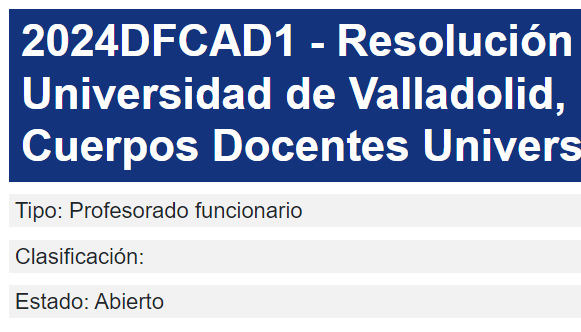
\includegraphics[width=0.75\linewidth]{DocumentacionTFG//img/CamposVaciosUVA.PNG}
    \caption{Convocatorias con campos vacíos}
\end{figure}

Estos han sido algunos inconvenientes a la hora de recopilar los datos de las distintas universidades. Todos ellos se han tratado de solventar de la manera más lógica posible intentando que afecten de la manera más mínima a la idea de aplicación que se tenía en el inicio.

\section{Integración con Calendario Personal}

Para añadir funcionalidad extra a la aplicación, se decidió realizar una integración con Google Calendar, para ello, en primer lugar, se tenía que dar la posibilidad a los usuarios de iniciar sesión con Google. Esto se implementó mediante la autenticación basada en OAuth 2.0 lo cual permitía a los usuarios de mi aplicación web iniciar sesión mediante la utilización de las cuentas de Google ~\cite{oauth2:latex}. 

Posteriormente, cuando el proceso de autenticación estaba completado, se realizó un desarrollo para que los usuarios pudiesen añadir como evento, las fechas de fin de las convocatorias a Google Calendar desde la aplicación y de esta manera disponer de un recordatorio previo antes de que las convocatorias expirasen. Esta integración se intentó realizar mediante Google Cloud Console que permitía a los desarrolladores gestionar sus servicios en Google Cloud.

Esta integración con Google y Google Calendar, se acabó llevando a cabo y era funcional para usuarios de test, sin embargo, si se quería publicar la aplicación y que la integración fuese funcional para cualquier usuario, Google requería lo siguiente para completar el proceso de verificación:

\begin{itemize}
    \item Un enlace oficial a la Política de Privacidad de la aplicación
    \item Un vídeo de YouTube que muestra cómo 
 se planea utilizar los datos de usuario de Google que obtiene de los ámbitos.
    \item Una explicación escrita que le indique a Google por qué necesita acceso a datos de usuario confidenciales y/o restringidos.
    \item Todos tus dominios verificados en Google Search Console
\end{itemize}

Estas restricciones, fueron consideradas demasiado duras como para un proyecto de este calibre. Además, quizás esta integración limitaba el disfrute de la funcionalidad de la aplicación para aquellos usuarios que no dispusiesen de cuenta de Google, por lo tanto se decidió cambiar esta funcionalidad y se implementó un nuevo sistema de avisos por correo.

\textbf{Nuevo Sistema de Avisos por Correo}

Para este sistema de avisos implementado, los usuarios no tenían necesariamente que iniciar sesión con su cuenta de correo electrónico de manera inicial como anteriormente. 

Para la utilización de esta funcionalidad, bastará con que el usuario se suscriba al sistema de avisos de la convocatoria que el desee mediante un formulario en el que debe introducir su correo electrónico. 

Una vez que se suscribe, le llegará al usuario un correo con información de la convocatoria solicitada y un archivo ICalendar definido por la aplicación. Estos archivos permiten añadir como evento a su calendario personal la fecha de fin de una convocatoria para que el usuario se acuerde del fin de plazo de la misma. Además, en este caso dará igual cual sea el servicio de correo electrónico utilizado (Google, Outlook...) lo cual mejora enormemente la implementación anterior.

\section{Despliegue de la aplicación}

La idea inicial para realizar el despliegue de la aplicación, era Docker ~\cite{docker:latex}. Esta es una herramienta que permite a los desarrolladores a crear, compartir, ejecutar y verificar aplicaciones en cualquier lugar sin complejas configuraciones del entorno. 

Sin embargo, cuando se utiliza Docker en Windows, es necesario tener habilitada alguna tecnología de virtualización, normalmente el Subsistema de Windows para Linux. Para ello, se necesita habilitar la característica WSL en mi ordenador lo cual era una operación que no acababa de completarse debido a errores en el camino. 

Tras varias pruebas, cambios en archivos de configuración, etc. Se decidió investigar otras herramientas para el despliegue. Esta decisión tomada, es algo que ha dado un salto de calidad al proyecto debido a que actualmente la aplicación está desplegada de una manera muy profesional y novedosa.

Los componentes fundamentales para el despliegue final de la aplicación han sido los siguientes:
\begin{itemize}
    \item \textbf{Servidor de Azure Database para MySQL: ~\cite{azuremysql:latex}} En este servidor en la nube, se ha desplegado la base de datos MySQL. Esta decisión se ha tomado de esta manera debido a la facilidad que nos proporciona Azure para realizar despliegues sin realizar tareas de infraesctructura.
    \item \textbf{GitHub Action:~\cite{githubactions:latex}} Esta herramienta es utilizada para la automatización de flujos de trabajo. En el sistema, se ha utilizado esta herramienta para crear una tarea programada que ejecutará el proyecto en Python y por lo tanto hará que la base de datos se actualice de manera periódica.
    \item \textbf{Azure App Services: ~\cite{azureappservices:latex}} Este es un servicio basado en HTTP que permite hospedar aplicaciones web en la nube. En nuestro sistema, es el encargado de lanzar y alojar la aplicación desarrollada en .NET en la nube. Esto fue sencillo debido a que tanto Azure como .NET son propias de Microsoft por lo tanto el despliegue se pudo realizar con facilidad. Para que la información de la base de datos se mostrase correctamente en la web desplegada, se tuvieron que configurar las variables de entorno de este App Service e introducir la cadena de conexión de la base de datos desplegada en el servidor Azure Database. Este fue el último paso del montaje de la arquitectura del sistema y por lo tanto ya estaba la aplicación funcional disponible para utilizarse. 
\end{itemize}

\newpage
\begin{landscape}
\subsubsection{Diagrama de arquitectura general del sistema desplegado}
\vspace{2cm}
\imagenapaisada{DiagramaGeneralArquitectura}{Diagrama arquitectura general del sistema.}\label{img-diagrama-general}   
\end{landscape}
\newpage









\capitulo{6}{Trabajos relacionados}

Aunque no se disponga de información sobre si se han realizado proyectos previos sobre recopilación de convocatorias del PDI y PAS de manera centralizada y, tampoco se ha encontrado información en la web sobre su existencia. Voy a utilizar este apartado para exponer algunas aplicaciones web interesantes en las que se utiliza \textit{web scraping} para la recopilación de datos y posteriormente mostrarlos en la web.

\section{Indeed}
Indeed es una plataforma que permite a los usuarios buscar empleos, guardarlos y solicitarlos directamente. En esta web se incluyen todas las ofertas de empleo de las principales bolsas, periódicos, asociaciones y páginas de empleo de las empresas. Todos los datos de estas ofertas son recopilados mediante \textit{web scraping} a todas estas plataformas que se encargan de publicar empleos diariamente.

Este modelo de aplicación es un modelo muy parecido al de la aplicación del proyecto dado que se tiene el mismo objetivo: Mostrar en una misma página web las ofertas de una manera centralizada. 

La principal diferencia entre la aplicación web Indeed y DeltaOffers, es que Indeed está destinada a fines más comerciales mientras que DeltaOffers lo que pretende es servir a la comunidad universitaria.

\section{Chollometro}
Chollometro es una aplicación web que se encarga de la recopilación de ofertas, cupones y promociones disponibles en tiendas \textit{online} y físicas.

Para la recopilación de todos estos descuentos en productos, esta aplicación también realiza \textit{web scraping} de otras webs. 

Esta aplicación, al igual que DeltaOffers, se encarga de recopilar datos (en este caso sobre descuentos) para mostrarlos a los usuarios de una manera centralizada.

\section{Google News}
Google News es una plataforma la cual muestra noticias de la actualidad. Estas noticias provienen de otros periódicos o fuentes de información y Google News las muestra de manera actualizada.

Al igual que en los casos anteriores, esta página web utiliza \textit{web scraping} para la recopilación de noticias y las muestra en su propia web de manera unificada.

\capitulo{7}{Conclusiones y Líneas de trabajo futuras}

En este apartado de van a detallar cuales son las conclusiones a destacar una vez finalizado el proyecto. Además, se va a realizar un informe crítico sobre cómo es posible mejorar el proyecto y continuar en la línea de lo realizado hasta ahora.

\section{Conclusiones}
En cuanto al resultado final del proyecto, puedo destacar que estoy enormemente satisfecho por el cumplimiento de los objetivos propuestos inicialmente. Se ha conseguido desarrollar una aplicación que muestra las convocatorias de manera centralizada y actualizada y, además se ha proporcionado una mayor funcionalidad a la misma.

Durante el transcurso de este proyecto, he podido aprender gran variedad de técnicas y herramientas que me van a ser de provecho para el futuro. Actualmente, poseo muchos más conocimientos en comparación con mis inicios en el proyecto lo cual es algo que me llena de orgullo.

Además, dado que se ha trabajado de manera autodidacta, creo que este trabajo también me ha ayudado a convertirme en una persona mucho más resolutiva y eficaz en situaciones complicadas.

Por último, me gustaría destacar la motivación que este proyecto me ha aportado para continuar mi desarrollo en el mundo del software.


\section{Líneas de trabajo futuras}
En el caso de que este proyecto continúe adelante, se van a indicar en este apartado las líneas de trabajo próximas para los futuros desarrolladores del mismo:

\begin{itemize}
    \item Para que la aplicación responda ante las interacciones del usuario de manera más rápida, podría ser interesante un cambio de despliegue a un servidor de pago. Esto se debe a que actualmente la aplicación está desplegada en servidores gratuitos los cuales tienen unas características mucho más limitadas.
    \item Para aumentar el alcance de la aplicación web, sería interesante comenzar a recopilar las convocatorias de más universidades de España y empezar a mostrar esas convocatorias en la web para llegar a un mayor número de usuarios.
    \item En el caso de que se quisiese realizar una aplicación más profesional en Castilla Y León, se podría intentar contactar con las universidades para contar con su apoyo frente al proyecto y que las convocatorias que se empiecen a subir a sus propias webs posean un formato sólido y estructura unificada.
    \item Por último, sería interesante continuar con la implementación de nuevas funcionalidades en la aplicación.
\end{itemize}


\bibliographystyle{plain}
\bibliography{bibliografia}

\end{document}
